%% %%%%%%%%%%%%%%%%%%%%%%%%%%%%%%%%%%%%%%%%%%%%%%%%
%% Problem Set/Assignment Template to be used by the
%% Food and Resource Economics Department - IFAS
%% University of Florida's graduates.
%% %%%%%%%%%%%%%%%%%%%%%%%%%%%%%%%%%%%%%%%%%%%%%%%%
%% Version 1.0 - November 2019
%% %%%%%%%%%%%%%%%%%%%%%%%%%%%%%%%%%%%%%%%%%%%%%%%%
%% Ariel Soto-Caro
%%  - asotocaro@ufl.edu
%%  - arielsotocaro@gmail.com
%% %%%%%%%%%%%%%%%%%%%%%%%%%%%%%%%%%%%%%%%%%%%%%%%%

\documentclass[12pt]{article}
\usepackage{design_ASC}

\usepackage{tikz}
\usetikzlibrary{automata, positioning, arrows}
\tikzset{
->, % makes the edges directed
node distance=3cm, % specifies the minimum distance between two nodes. Change if necessary.
every state/.style={thick, fill=gray!10}, % sets the properties for each ’state’ node
initial text=$ $, % sets the text that appears on the start arrow
}

\setlength\parindent{0pt} %% Do not touch this

%% -----------------------------
%% TITLE
%% -----------------------------
\title{Homework \#1} %% Assignment Title

\author{Artemis Kelly\\ %% Student name
CS424 - Theory of Computation\\ %% Code and course name
}

\date{\today} %% Change "\today" by another date manually
%% -----------------------------
%% -----------------------------

%% %%%%%%%%%%%%%%%%%%%%%%%%%
\begin{document}
\setlength{\droptitle}{-5em}    
%% %%%%%%%%%%%%%%%%%%%%%%%%%
\maketitle

% --------------------------
% Start here
% --------------------------

% %%%%%%%%%%%%%%%%%%%
\section*{Question 1.6}
% %%%%%%%%%%%%%%%%%%%
 Give state diagrams of DFAs recognizing the following languages. In all parts, the alphabet is \{0,1\}

% %%%%%%%%%%%%%%%%%%%
\subsection*{Question 1: 1.6b}
% %%%%%%%%%%%%%%%%%%%
{\bfseries Question:} \{w $\|$ w contains at least three 1s\}

\begin{figure}[ht] % ’ht’ tells LaTeX to place the figure ’here’ or at the top of the page
\centering % centers the figure
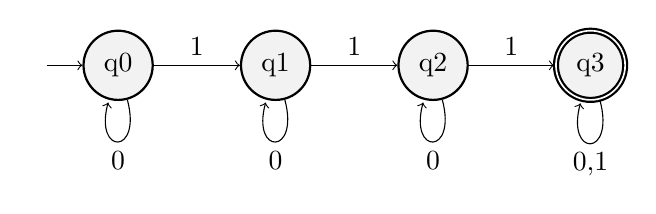
\begin{tikzpicture}

\node[state, initial] at (0, 0) (q0) {q0};
\node[state] at (2, 0) (q1) {q1};
\node[state] at (4,0) (q2) {q2};
\node[state, accepting] at (6,0) (q3) {q3};

\draw (q0) edge[above] node{1} (q1);
\draw (q1) edge[above] node{1} (q2);
\draw (q2) edge[above] node{1} (q3);
\draw (q0) edge[loop below] node{0} (q0);
\draw (q1) edge[loop below] node{0} (q1);
\draw (q2) edge[loop below] node{0} (q2);
\draw (q3) edge[loop below] node{0,1} (q3);
\end{tikzpicture}
\caption{DFA}
\label{fig:question 1}
\end{figure}

% %%%%%%%%%%%%%%%%%%%
\subsection*{Question 2: 1.6c}
% %%%%%%%%%%%%%%%%%%%
{\bfseries Question:} \{w $\|$ w contains the substring 0101 (i.e., w = x0101y for some x and y)\} 

\begin{figure}[ht] % ’ht’ tells LaTeX to place the figure ’here’ or at the top of the page
\centering % centers the figure
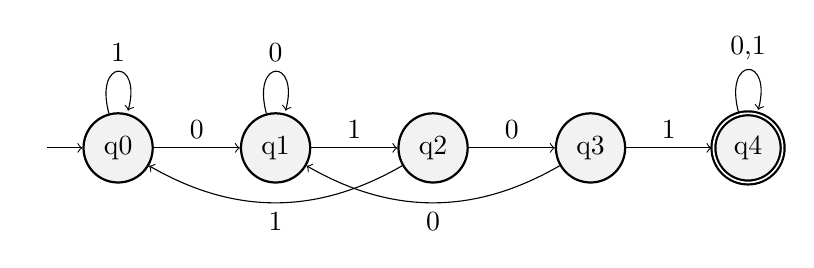
\begin{tikzpicture}

\node[state, initial] at (0, 0) (q0) {q0};
\node[state] at (2, 0) (q1) {q1};
\node[state] at (4,0) (q2) {q2};
\node[state] at (6,0) (q3) {q3};
\node[state, accepting] at (8,0) (q4) {q4};

\draw (q0) edge[above] node{0} (q1);
\draw (q1) edge[above] node{1} (q2);
\draw (q2) edge[above] node{0} (q3);
\draw (q3) edge[above] node{1} (q4);

\draw (q1) edge[loop above, above] node{0} (q1);
\draw (q0) edge[loop above] node{1} (q0);

\draw (q2) edge[bend left, below] node{1} (q0);
\draw (q3) edge[bend left, below] node{0} (q1);
\draw (q4) edge[loop above] node{0,1} (q4);

\end{tikzpicture}
\caption{DFA}
\label{fig:question 2}
\end{figure}

% %%%%%%%%%%%%%%%%%%%
\subsection*{Question 3: 1.6f}
% %%%%%%%%%%%%%%%%%%%
{\bfseries Question: } \{w $\|$ w doesn’t contain the substring 110\}

\begin{figure}[ht] % ’ht’ tells LaTeX to place the figure ’here’ or at the top of the page
\centering % centers the figure
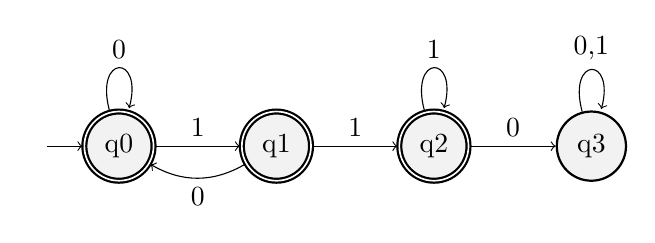
\begin{tikzpicture}

\node[state, initial, accepting] at (0, 0) (q0) {q0};
\node[state, accepting] at (2, 0) (q1) {q1};
\node[state, accepting] at (4,0) (q2) {q2};
\node[state] at (6,0) (q3) {q3};

\draw (q0) edge[above] node{1} (q1);
\draw (q1) edge[above] node{1} (q2);
\draw (q2) edge[above] node{0} (q3);

\draw (q3) edge[loop above, above] node{0,1} (q3);
\draw (q2) edge[loop above, above] node{1} (q2);
\draw (q1) edge[bend left, below] node{0} (q0);
\draw (q0) edge[loop above, above] node{0} (q0);

\end{tikzpicture}
\caption{DFA}
\label{fig:question 3}
\end{figure}

% %%%%%%%%%%%%%%%%%%%
\section*{Question 1.8}
% %%%%%%%%%%%%%%%%%%%
{\bfseries Question} Use the construction in the proof of Theorem 1.45 to give the state diagrams of NFAs recognizing the union of the languages described in.

% %%%%%%%%%%%%%%%%%%%
\subsection*{Question 4: 1.8b}
% %%%%%%%%%%%%%%%%%%%
{\bfseries Exercises 1.6c and 1.6f. }

\begin{figure}[ht] % ’ht’ tells LaTeX to place the figure ’here’ or at the top of the page
\centering % centers the figure
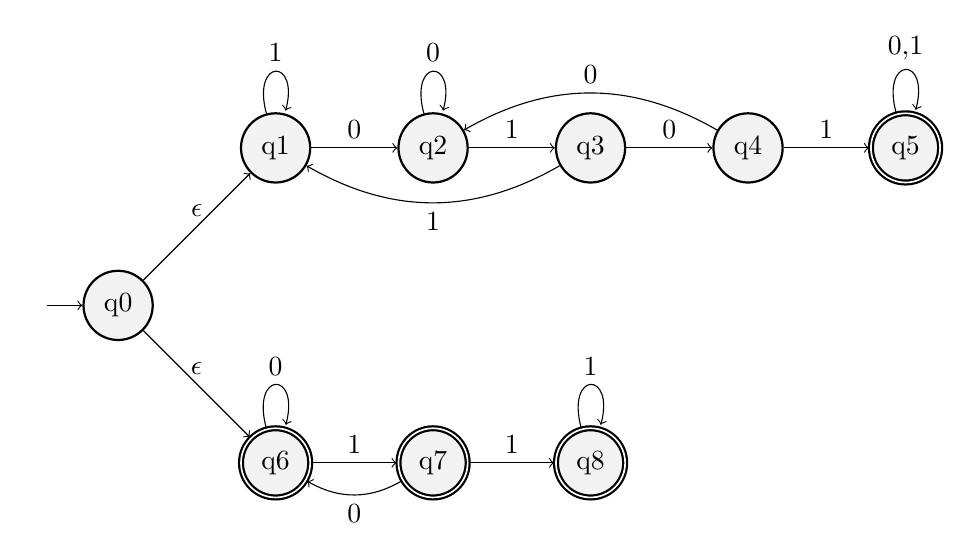
\begin{tikzpicture}

\node[state, initial] at (0, 0) (q0) {q0};
\node[state] at (2, 2) (q1) {q1};
\node[state] at (4,2) (q2) {q2};
\node[state] at (6,2) (q3) {q3};
\node[state] at (8,2) (q4) {q4};
\node[state, accepting] at (10,2) (q5) {q5};

\node[state, accepting] at (2,-2) (q6) {q6};
\node[state, accepting] at (4,-2) (q7) {q7};
\node[state, accepting] at (6,-2) (q8) {q8};

\draw (q0) edge[above] node{$\epsilon$} (q1);
\draw (q0) edge[above] node{$\epsilon$} (q6);
\draw (q1) edge[above] node{0} (q2);
\draw (q2) edge[above] node{1} (q3);
\draw (q3) edge[above] node{0} (q4);
\draw (q4) edge[above] node{1} (q5);
\draw (q5) edge[loop above, above] node{0,1} (q5);
\draw (q2) edge[loop above, above] node{0} (q2);
\draw (q3) edge[bend left,below] node{1} (q1);
\draw (q4) edge[bend right,above] node{0} (q2);
\draw (q1) edge[loop above, above] node{1} (q1);

\draw (q6) edge[above] node{1} (q7);
\draw (q7) edge[above] node{1} (q8);
\draw (q7) edge[bend left, below] node{0} (q6);
\draw (q8) edge[loop above, above] node{1} (q8);
\draw (q6) edge[loop above, above] node{0} (q6);

\end{tikzpicture}
\caption{NFA Combiation}
\label{fig:question 4}
\end{figure}

% %%%%%%%%%%%%%%%%%%%
\section*{Question 5: 1.10}
% %%%%%%%%%%%%%%%%%%%
{\bfseries Question:} Use the construction in the proof of Theorem 1.49 to give the state diagrams of NFAs recognizing the star of the languages described in 

% %%%%%%%%%%%%%%%%%%%
\subsection*{Question 1.10a}
% %%%%%%%%%%%%%%%%%%%
 Exercise 1.6b

\begin{figure}[ht] % ’ht’ tells LaTeX to place the figure ’here’ or at the top of the page
\centering % centers the figure
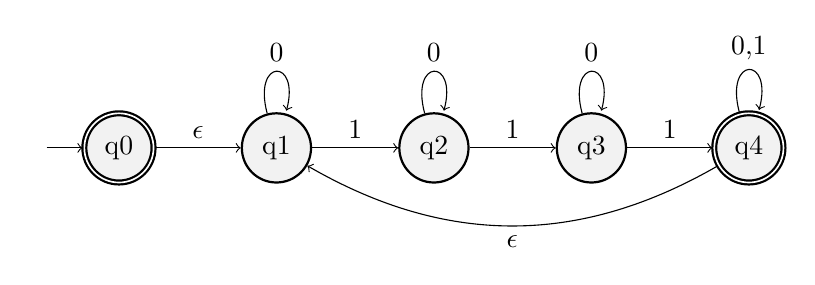
\begin{tikzpicture}

\node[state, initial, accepting] at (0, 0) (q0) {q0};
\node[state] at (2, 0) (q1) {q1};
\node[state] at (4, 0) (q2) {q2};
\node[state] at (6, 0) (q3) {q3};
\node[state,accepting] at (8, 0) (q4) {q4};

\draw (q0) edge[above] node{$\epsilon$} (q1);
\draw (q1) edge[above] node{1} (q2);
\draw (q2) edge[above] node{1} (q3);
\draw (q3) edge[above] node{1} (q4);

\draw (q1) edge[loop above, above] node{0} (q1);
\draw (q2) edge[loop above, above] node{0} (q2);
\draw (q3) edge[loop above, above] node{0} (q3);
\draw (q4) edge[loop above, above] node{0,1} (q4);
\draw (q4) edge[bend left, below] node{$\epsilon$} (q1);

\end{tikzpicture}
\caption{NFA Recognizing language of 1.6b}
\label{fig:question 5}
\end{figure}

% %%%%%%%%%%%%%%%%%%%
\section*{Question 6: 1.16}
% %%%%%%%%%%%%%%%%%%%
 Use the construction given in Theorem 1.39 to convert the following two non deterministic finite automata to equivalent deterministic finite automata.

% %%%%%%%%%%%%%%%%%%%
\subsection*{Question 1.16b}
% %%%%%%%%%%%%%%%%%%%
{\bfseries Question: } The NFA shown in the book has 3 states. Therefore, the DFA we can construct, which will accept the same language, must have $2^3$ states.

\begin{figure}[ht] % ’ht’ tells LaTeX to place the figure ’here’ or at the top of the page
\centering % centers the figure
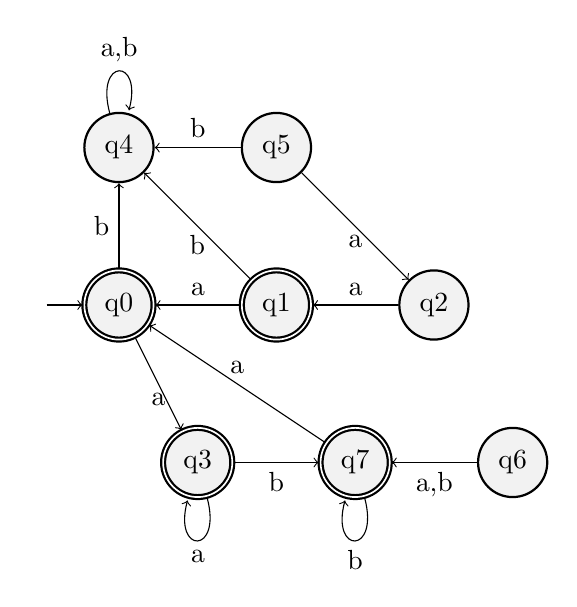
\begin{tikzpicture}

\node[state, initial, accepting] at (0, 0) (q0) {q0};
\node[state, accepting] at (2, 0) (q1) {q1};
\node[state] at (4, 0) (q2) {q2};
\node[state, accepting] at (1, -2) (q3) {q3};
\node[state] at (0, 2) (q4) {q4};
\node[state] at (2, 2) (q5) {q5};
\node[state] at (5, -2) (q6) {q6};
\node[state, accepting] at (3, -2) (q7) {q7};

\draw (q0) edge[left] node{b} (q4);
\draw (q1) edge[above] node{a} (q0);
\draw (q2) edge[above] node{a} (q1);
\draw (q0) edge[ below] node{a} (q3);
\draw (q3) edge[below] node{b} (q7);
\draw (q6) edge[below] node{a,b} (q7);
\draw (q7) edge[loop below, below] node{b} (q7);
\draw (q5) edge[above] node{b} (q4);
\draw (q4) edge[loop above, above] node{a,b} (q4);
\draw (q1) edge[below] node{b} (q4);
\draw (q5) edge[below] node{a} (q2);
\draw (q7) edge[above] node{a} (q0);
\draw (q3) edge[loop below, below] node{a} (q3);

\end{tikzpicture}
\caption{NFA Recognizing language of 1.6b}
\label{fig:question 6}
\end{figure}

% %%%%%%%%%%%%%%%%%%%
\section*{Question 7: 1.21}
% %%%%%%%%%%%%%%%%%%%
{\bfseries Question: }Use the procedure described in Lemma 1.60 to convert the following finite automata to regular expressions. 


% %%%%%%%%%%%%%%%%%%%
\subsection*{Question 1.21b}
% %%%%%%%%%%%%%%%%%%%
{\bfseries Answer:} The regular expression for the finite automata is $\epsilon$$|$(a$|$b)(a$|$bb$|$ba(a$|$b))*(b$|$ba). This is found by adding an additional start state with an $\epsilon$ transition to the beginning of the finite automata and then going through to get rid of states one at a time until you are left with a single transition, a start state and an accepting state.

% %%%%%%%%%%%%%%%%%%%
\section*{Question 8: 1.30}
% %%%%%%%%%%%%%%%%%%%
{\bfseries Question:} Describe the error in the following “proof” that $0^{*}$$1^{*}$is not a regular language. (An error must exist because $0^{*}$$1^{*}$is regular.) The proof is by contradiction. Assume that $0^{*}$$1^{*}$ is regular. Let p be the pumping length for $0^{*}$$1^{*}$ given by the pumping lemma. Choose s to be the string $0^p$$1^p$. You know that s is a member of $0^{*}$$1^{*}$, but Example 1.73 shows that s cannot be pumped. Thus you have a contradiction. So $0^{*}$$1^{*}$ is not regular. 
\\

{\bfseries Answer: } Lets call the language described above L. Looking at example 1.73, 1 and 2 are not relevant. The error in this proof is that using a single string as a counter example to show one language is non regular does not mean that every language which accepts that string is non regular. While the string xz would contain fewer zeros than ones, that is still in the language L because we do not need the same amount of zeros or ones.


% %%%%%%%%%%%%%%%%%%%
\section*{Question 9: 1.36}
% %%%%%%%%%%%%%%%%%%%
{\bfseries Question:} Let Bn = \{$a^k$  $\|$  k is a multiple of n\}. Show that for each n$\geq$ 1, the language Bn is regular. 
\\

{\bfseries Answer}: 
We build a DFA with n states, $q_0$, $q_1$ ,... $q_{n-1}$. These will serve to count the number of consecutive a's modulo n (because for each a that is input, the "counter" increases by 1 as it moves to the next state). $q_0$ is the only accepting state, at which point there must be n a's, in which case k must be a multiple of n. If it is not, then the DFA will end in a non accepting state. Because there is a DFA which recognizes this language, it must be a regular language. 

% %%%%%%%%%%%%%%%%%%%
\section*{Question 10: 1.42}
% %%%%%%%%%%%%%%%%%%%
{\bfseries Question:} For languages A and B, let the shuffle of A and B be the language.
\{w $\|$ w = $a_1$$b_1$ ... $a_k$$b_k$, where $a_1$ ... $a_k$  $\in$ A and $b_1$...$b_k$ $\in$ B, each $a_i$,$b_i$ $\in$  $\Sigma^{*}$ \}. Show that the class of regular languages is closed under shuffle. 
\\
\\
{\bfseries {Answer}: }
To show using languages A and B that the class of regular languages is closed under shuffle, A and B must be regular languages. Therefore, there is a DFA that can describe each of them. Lets take $DFA_A$ to be ($Q_A$, $\Sigma$, $\delta_A$, $q_A$, $F_A$) and $DFA_B$ to be ($Q_B$, $\Sigma$, $\delta_B$, $q_B$, $F_B$). We will use DFA S to be (Q, $\Sigma$, $\delta$, q, F), to describe the shuffle of A and B. 
\\
\\{\bfseries 1)} Q = $Q_A$ x $Q_B$ U {$q_0$}, $Q_A$ x $Q_B$ gives us all of the possible states of $DFA_A$ and $DFA_B$ and {$q_0$} is the start state
\\
\\{\bfseries 2)} q = $q_0$ 
\\
\\{\bfseries 3)}$\delta$ must describe that if the current state is in $DFA_A$, then the next input symbol must be in $DFA_B$ and vice versa. We only need to change the current state of the DFA which is reading an input symbol. So $\delta$((x,y,A)a) = ($\delta_A$(x,a),y,B) and vice versa $\delta$((x,y,B)b) = (x, $\delta_B$(y,a)A)
$\delta$ must work with transitions for 3 different scenarios. First, $\delta$($q_0$, $\epsilon$) = ($q_A$,$q_B$). This means that at the start state, both $DFA_A$ and $DFA_B$ can go to their start states without reading anything in. Second, ($\delta_A$(x,a),y) \in $\delta$((x,y),a). This means that if we read in a character that should move $DFA_A$ to the next state, we can do so accordingly without changing the state of $DFA_B$. Lastly, we have the opposite in which case the next input character is used to change the state of $DFA_B$ and not $DFA_A$. (x,$\delta_B$(y,a)) \in $\delta$((x,y),a).
\\
\\{\bfseries 4)} S will accept the input string if both $DFA_B$ and $DFA_A$ are in the accept states. It will also accept the empty string, at which case the input will have ended with S in its start state  F = $F_A$ x $F_B$ U {$q_0$}
\\
\\
The DFA which recognizes the shuffle can alternate between an input character recognized by $DFA_A$ to an input character recognized by $DFA_B$ as each character is read in, but does not have to. Therefore, S must keep track of which state $DFA_A$ is in and which state $DFA_B$ is in so that when it takes it's next input character, it can see which DFA to move accordingly. When it recognizes which DFA's state to switch, it must switch appropriately.  When the entirety of the input is processed, if both $DFA_A$ and $DFA_B$ are in accept states, then the input string is accepted and S can accept. Because there is a DFA that describes the regular language of the shuffle of regular languages A and B, the shuffle itself is also a regular language. 



\end{document}